%\section{数据、信息与进位制}
\setcounter{section}{1}
\setcounter{subsection}{2}
\subsection{1.5 ASCII编码、大数据}



\begin{compactenum}[1.]
%\labelwidth = 2em
\item \textbf{数据的定义}
	\begin{compactitem}
	\item 数据是对客观事物的符号表示。
	\item 在计算机科学中,数据表现形式可以是文字、图形、图像、音频、视频等。
	\end{compactitem}
\item \textbf{信息及信息的特征}
	\begin{compactitem}
	\item 信息是数据、信号中所包含的含义
	\item 信息具有\textbf{载体依附性}、时效性、共享性、可加工处理性等特征。
	\end{compactitem}
\item \textbf{知识}
	\begin{compactitem}
	\item 知识是人类在社会实践中所获得的认识和经验的总和,也是人类在实践中认识客观世界的成果,它包括对事实、信息的描述及在教育和实践中获得的技能。
	\item 知识是可以积累与传承的。
	\end{compactitem}
\item \textbf{数据、信息与知识的关系}
	\begin{compactitem}
	\item 数据经过解释后产生的意义就是信息,数据是信息的载体,单纯的数字是没有意义。
	\item 通过归纳、演绎、比较等手段对信息进行挖掘,将万千信息中有价值的部分与已存在的人类知识体系相结合,形成知识。
	\item 数据、信息与知识的关系可以通过图表示
	\end{compactitem}
\begin{figure}[!ht]
\centering
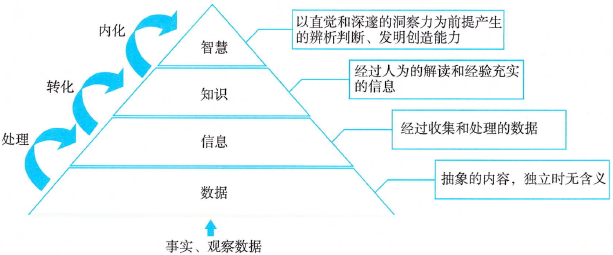
\includegraphics[width=0.5\linewidth]{pic/c01.01.info.knowledge}
\end{figure}


\item \textbf{数字化}
	\begin{compactitem}
	\item 将模拟信号转换为数字信号的过程称为数字化
	\item 将模拟信号转换成数字信号一般需要经过采样、量化与编码
	\end{compactitem}

\item \textbf{进制转换}
	\begin{compactitem}
	\item 将\underline{十进制$ \to k$进制}:\textbf{除$k$取余法},将\underline{$k$进制$\to$十进制}数可用\textbf{按权相加法}(即$\times \; k^{i-1}$),e.g.
		\begin{compactitem}[\ding{86}]
		\item $25D$=$11001B, \because $
		\[ \begin{aligned} 25 \div 2=12\cdots & {\color{red}1} \\
		12 \div 2=6\cdots & {\color{red}0} \\
		6 \div 2=3\cdots & {\color{red}0} \\
		3 \div 2=1\cdots & {\color{red}1} \\
		1 \div 2=0\cdots & {\color{red}1}
		\end{aligned} \]
		\item $D2H=208D, \because 13\times 16^1 + 2 \times 16^0=208$
		\end{compactitem}
	
	\item 二进制数转换成十六进制数,从二进制数的低位开始,每四位二进制数转换成一位十六进制数;反之,每一位十六进制数可转换成四位二进制数。e.g.
		\begin{compactitem}[\ding{86}]
		\item $D2H = 11010010B, \because \; D_{(16)} \to 13_{(10)} \to 1101_{(2)}, 2_{(16)} \to 2_{(10)} \to 11_{(2)}$
		\item $110111B = 37H, \because \; 0111_{(2)} \to 7_{(10)} \to 7_{(16)}, 11_{(2)} \to 3_{(10)} \to 3_{(16)}$
		\end{compactitem}
	\end{compactitem}

\end{compactenum}%


\begin{groups}


\group{单选题}{每题仅有一个正确选项}
\begin{questions}[rp]

%% =========== 1
\question
\smkai{(作业本1.3)}下列有关ASCII编码的说法,正确的是
\choice{共有127个字符}
{每个字符用1个字节中的高7位编码}
{每个字符占用1个字节的存储空间}
{可以用于汉字字符的编码}
\begin{solution}
C。标准的ASCII码共128个,每个字符用1个字节中的低7位进行编码,在计算机中,一般以字节为单位存储数据,故每个ASCI字符占用1个字节的存储空间,ASCII编码不能用于汉字编码。
\end{solution}

%% =========== 2
\question
\smkai{(作业本1.3)}下列不属于字符编码的是
\choice{ASCII}
{Unicode}
{GB2312}
{GIF}
\begin{solution}
D。ASCII , Unicode ,GB2312均为字符编码;GIF是图像编码。
\end{solution}

%% =========== 3
\question
\smkai{(作业本1.3)}下列单位换算正确的有①$1Byte=8bit$ ②$1KB=8Byte$ ③$1MB=1024KB$ ④$1GB=1024Byte$
\choice{①②}
{①③}
{②③}
{②④}
\begin{solution}
B。
\end{solution}

%% =========== 4
\question
\smkai{(作业本1.3)}在计算机中表示1个GB2312汉字字符需要
\choice{1个字节}
{2个字节}
{3个字节}
{4个字节}
\begin{solution}
B。GB2312汉字采用双字节编码,所以编码1个字符需用2个字节。
\end{solution}

%% =========== 5
\question
\smkai{(作业本1.3)}在计算机中,用于存储汉字的编码是
\choice{ASCII码}
{机内码}
{拼音码}
{五笔字形码}
\begin{solution}
B。ASCII码用于表示现代英语和其他西欧语言,汉字在计算机内部以机内码存储,拼音码和五笔字形码属于汉字的输入码。
\end{solution}

%% =========== 6
\question
\smkai{(作业本1.3)}条形码的最后1位(最右边1位)数字为校验码,其计算方式为:
(1)将条形码编码数字包括校验码在内,按由右至左的顺序进行编号,校验码的代码位置序号为1。
(2)校验码的计算步骤如下:
①从编码位置序号2开始,对所有偶数位的编码数字求和,将得到的和乘以3;
②从编码位置序号3开始.对所有奇数位的编码数字求和;
③将步骤①与步骤②的结果相加,仅保留其个位数字;
④用10减去步骤③的结果,其差的个位数字即为所求校验码的值
现有条形码,其编码数字为$978-7-04-049606-X$,其中$X$为校验码。则该值是
\choice{0}
{2}
{4}
{8}
\begin{solution}
B。计算公式:$(6+6+4+4+7+7)*3+(0+9+0+0+8+9)=128$,再用10减去8得2。
\end{solution}

%% =========== 7
\question
\smkai{(作业本1.5)}下列关于数据与大数据的说法正确的是
\choice{数据是现代科学研究的重要资源}
{大数据的数据量庞大,价值密度高}
{计算机中的数据都以ASCII码存储}
{大数据的应用降低了用户隐私信息泄露的风险}
\begin{solution}
A。科学研究离不开数据,数据是科学研究的重要资源:大数据的数据量庞大,所以其价值密度相对较低:计算机中的数据以二进制形式存储,ASCII码是一种字符的编码方式;大数据的应用加大了用户隐私信息泄露的风险。
\end{solution}

%% =========== 8
\question
\smkai{(作业本1.5)}我们每天都在跟各类软件打交道:聊天、购物、看新闻和短视频每一次我们的点击和滑动都会成为数据的一部分,有关组织通过数据的搜集、存储、分析和可视化技术,解决大数据海量、高速、多变、价值密度低的问题,使数据从散乱的信息变成知识和智慧帮助组织解决发展中遇到的实际问题,对于上述描述。下列说法不正确的是
\choice{你的每次上网行为及相关数据可能会被采集}
{你在上网时的每次操作,蕴含着巨大的价值}
{你在聊天、购物、看新闻和短视频等过程中,有可能泄露个人隐私}
{网站提供给你的“个性化推荐”,依赖于你的上网行为}
\begin{solution}
B。本题中的大数据来源于人们日常的信息获取、交流等行为,在人们聊天、购物、浏览网页等操作时,会不经意间发布各种数据,并留下操作痕迹,这些数据会被记录、累积下来。在这些数据中。有些数据可能会泄露个人隐私。如网上填报的实名信息,发布的冬片中可能含有GPS信息等。相关机构将这些数据采集后,有可能挖掘出有价值的数据,但并不是用户的每次上网行为都有价值。如用户的随意点击等,所以答案是B
\end{solution}

%% =========== 9
\question
\smkai{(作业本1.5)}关于大数据的特征和大数据对社会影响,说法正确的是
\choice{大数据的特征主要包括数据量大、速度快、数据类型多、价值密度低}
{大数据消除数字鸿沟和信息不对称}
{大数据价值密度低,降低了信息泄露的风险}
{大数据数据量大,给人们的生活带来了不便}
\begin{solution}
A。大数据的应用促进经济发展和创新,给人们生活带来便利,同时会加剧数学鸿沟,增加信点泄露风险
\end{solution}

%% =========== 10
\question
\smkai{(作业本1.5)}下列数据中属于大数据的是:①社交平台上产生的数据,②交通摄像头记录的数据,③某校历次考试成绩数据,④电商平台交易数据
\choice{①②③}
{①②④}
{①③④}
{②③④}
\begin{solution}
B。校的历次考试数据体量小、数据类型单一,显然不属于大数据;①②④都属丁大数据的典型应用。
\end{solution}

%% =========== 11
\question
\smkai{(作业本1.5)}下列有关大数据的说法,正确的是
\choice{大数据可以对全体数据进行分析}
{在大数据时代,样本数据分析法已经不再使用}
{大数据采集的数据以结构化数据为主}
{用大数据进行数据处理时,必须保证每个数据都准确无误}
\begin{solution}
A。大数据一般分析全样本数据;是否采用全样本数据分析还是抽象数据分析方法,需要根据实际情况而定:大数据米集的数据以非结构化,半结构化数据为主:大数据处理时,不需要保证每个数据都准确无误。
\end{solution}

%% =========== 12
\question
\smkai{(作业本1.5)}某用户在网上购买了一件商品,电商根据交易平台的大数据,给该用户进行个性化推荐时,最不需要考虑的是
\choice{该商品一般与什么商品组合销售}
{购买过该商品的其他用户还会购买什么商品}
{该用户曾经购买过什么产品}
{该用户为什么购买这件商品}
\begin{solution}
D。解析:大数据分析用户购买商品往往不需要考虑每个用户的购买原因,而是注重商品之间的相关性,所以答案是D。
\end{solution}






\end{questions}
\end{groups}
